\subsection{FPGA Interface} \label{subsec:FPGAInterface}
The Main Processor and Sample Control modules need a communication interface in order to set control settings for the ADCs, DAC in the FPGA's internal registers and to retrieve stored ADC samples.The ADCs and DAC \todo{Vi mangler at redegøre for det her valg.} both have 16 bits of resolution and a 16 bit wide parallel bus between the FPGA and MCU will be used to transfer the data as shown on figure \refq{fig_7_2_1_CommBus}.

\begin{figure}[H]
    \centering
    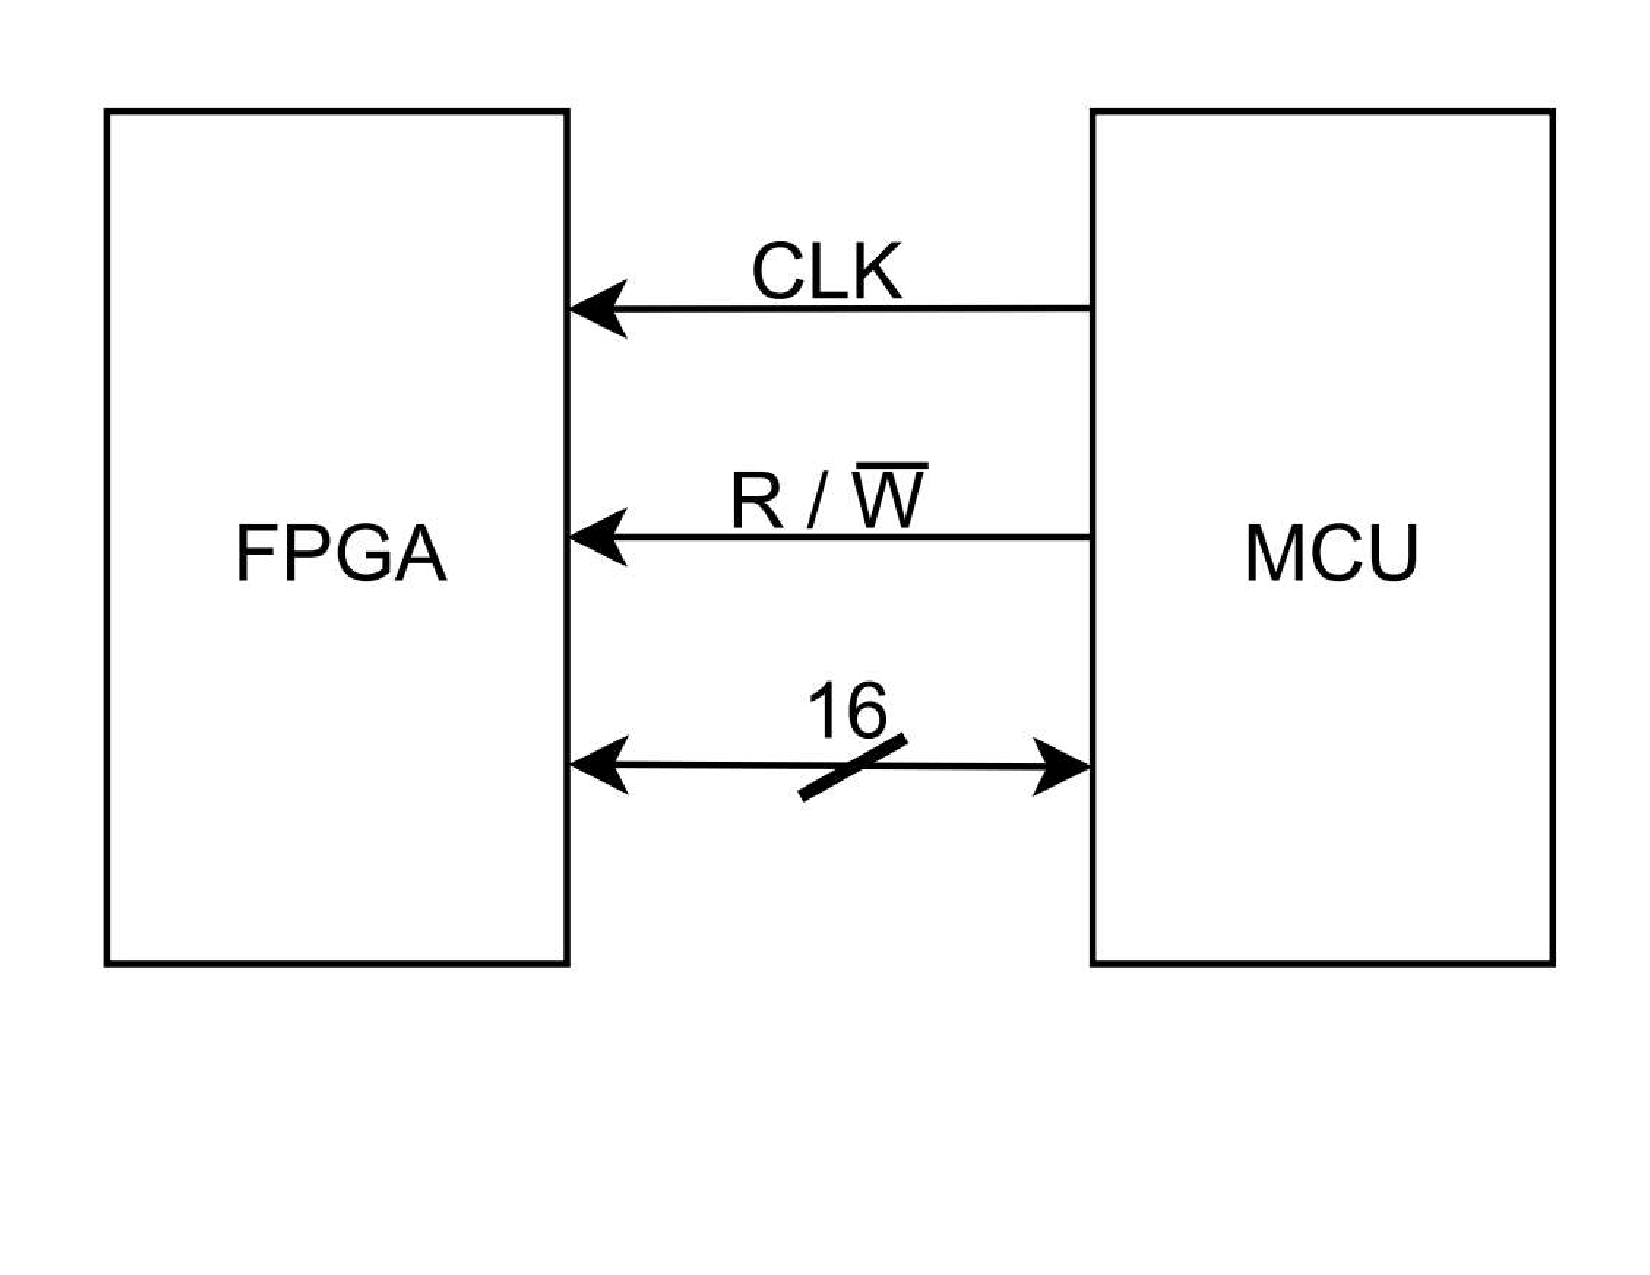
\includegraphics[clip, trim=0 100 0 0, width=0.5\textwidth]{Sections/7_SystemDesign/Figures/7_2_1_CommunicationBus.pdf}
    \caption{The communication bus connection the FPGA and microcontroller. It uses a 16 bit databus, a long with a CLK and a read/write control signal.}
    \label{fig_7_2_1_CommBus}
\end{figure}

The microcontroller is always going to be the master that has to initiate communication and the FPGA is always the slave. If the MCU wants to write some value into a register it must first write address into the FPGA followed by some value.